
\section {Introduction}

\begin{figure}[htp]
    \centering
    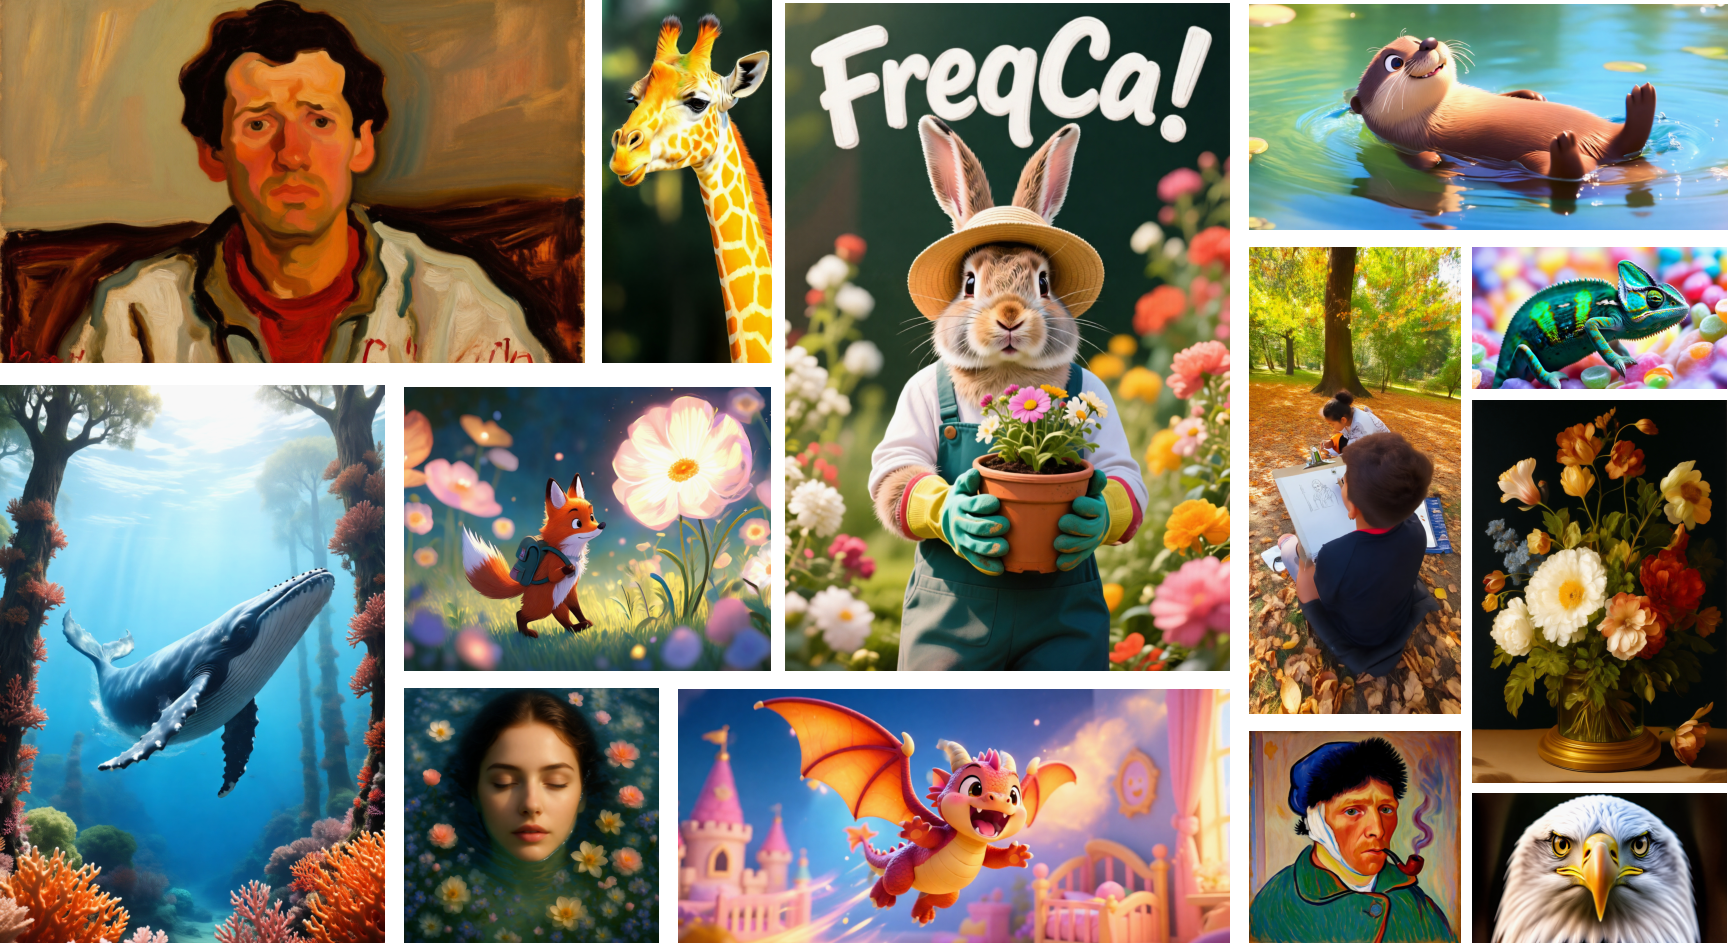
\includegraphics[width=0.9\linewidth]{figures/header_image.pdf}
    \caption{Images sampled by Qwen-image with \textit{FreqCa} with 7.14$\times$ acceleration. }
    \label{fig:showcase}
\end{figure}
\vspace{-3mm}   

\begin{figure}[htbp]
    \centering
    \includegraphics[width=\linewidth]
    {figures/analysis.pdf}
        \vspace{-6mm}
    \captionof{figure}{\textbf{Analysis from the frequency perspective.} \textbf{(a)-(b)}:Temporal similarity analysis using cosine similarity for low-frequency and high-frequency components across different step intervals. \textbf{(c)-(d)}: Feature trajectory visualized via Principal Component Analysis (PCA). }
    \label{fig:analysis}
    \vspace{-7mm}
\end{figure}



Diffusion Models (DMs) have achieved remarkable success in generative tasks like image synthesis and video generation \citep{DM,StableDiffusion,blattmann2023SVD}. The recent introduction of Diffusion Transformers \citep{DiT} has further advanced generation quality and diversity, establishing them as the predominant architecture for large-scale visual content creation. However, diffusion transformers typically rely on a stack of heavy transformer blocks and multi-step sampling, making computational efficiency a critical bottleneck for their practical deployment. 
To address this, the paradigm of feature caching has emerged, which exploits the high temporal redundancy between adjacent timesteps for acceleration~\citep{ma2024deepcache,li2023FasterDiffusion,selvaraju2024fora,chen2024delta-dit,zou2024accelerating,zou2024DuCa}. 


\textbf{The debate of caching paradigms.} Feature caching has gradually emerged into two different paradigms. The paradigm of ``Cache-Then-Reuse'' assumes that the features of DM in adjacent timesteps are highly \textbf{similar} and thus proposes to directly \textbf{reuse} the features of previous timesteps in the future timesteps~\citep{selvaraju2024fora}.  In contrast, the paradigm of ``Cache-Then-Forecast'' assumes that features of DM are ``continuous'' and thus proposes to forecast features in the future timesteps based on features in the previous timesteps with non-parametric predictors such as Taylor expansion. Although the paradigm ``Cache-Then-Forecast''    tends to show better performance in recent works, their assumption of continuity does not always hold perfectly. For instance, Liu~\emph{et al.} demonstrates that features of FLUX are not high-order continuous, making TaylorSeer degenerate into a linear prediction method and thus suffer from quality loss~\citep{liuTaylorSeer2025}. Based on these findings, this paper begins with an in-depth analysis of the temporal dynamics of diffusion models. 

\textbf{Analysis from the frequency perspective.} In classical image processing, the high-frequency and low-frequency components of images are usually considered as carrying different semantic information,  which motivates us to study the dynamics of high-frequency and low-frequency components in the feature of diffusion models separately. As shown in Figure~\ref{fig:analysis}(a)-(b), surprisingly, we find different frequency exhibits significantly different dynamics. Concretely, the similarity of low-frequency is higher than \emph{0.90} at most timesteps, while the high-frequency exhibits clearly low similarity.
%, indicating it is safe to directly reuse the previous low-frequency information
On the other hand, as shown in Figure~\ref{fig:analysis}(c)-(d), the feature trajectory of high-frequency shows perfect stability and continuity, while the feature trajectory of low-frequency is unstable and accompanied by sudden mutation, indicating that the high-frequency information can be accurately predicted while the low-frequency information fails.

Based on the above observations, this paper introduces \textbf{Freq}uency-aware Feature \textbf{Ca}ching (\textbf{FreqCa}), which aims to decouple the frequency of the features in diffusion models and treat them in different paradigms. Concretely, \textit{FreqCa} applies any frequency decomposition (\emph{e.g, Fourier Transformation}) to the cached features. For the low-frequency bands, we directly reuse them in the future timesteps because of their \emph{high similarity}. For the high-frequency bands, we predict their values in the future timesteps with any sequential predictor (\emph{Hermite polynomial predictor}) for their \emph{good continuity}. Then, in the future timesteps, \textit{FreqCa} reconstructs the features based on the reused low-frequency bands and predicted high-frequency bands,
enabling it to skip the computation over diffusion transformers, achieving the best cooperation between the previous caching paradigms.



%While these pioneering works validate the potential of temporal redundancy, their treatment of features as monolithic wholes represents a significant, unexplored avenue for optimization. A more fine-grained perspective is required, one that can meaningfully decompose features into distinct sub-components. To this end, we argue that a frequency-domain analysis provides the most natural and effective lens, as it inherently separates the low-frequency components governing global structure from the high-frequency components encoding fine-grained details.

%Temporal dynamics of feature frequency components. (a) Low-frequency components exhibit high temporal stability, while (b) high-frequency components are highly volatile, with similarity decaying rapidly as the step interval increases.
%Feature trajectory of high-frequency components obtained via PCA.





%Our quantitative investigation on FLUX reveals a critical, long-overlooked phenomenon: low-frequency components,  exhibit a smooth evolution with high consistency across time steps (Figure~\ref{fig:freq_similarity_analysis}(a)), making them ideal candidates for direct caching. High-frequency components, fluctuate dramatically, with their temporal similarity decaying rapidly as the step interval increases (Figure~\ref{fig:freq_similarity_analysis}(b)), thus forming the key bottleneck for quality degradation in existing caching methods. Further analysis reveals, however, that this high-frequency evolution is not random noise. Through Principal Component Analysis (PCA), we find their trajectories trace a smooth curve(Figure~\ref{fig:high_freq_pca}). This key insight reveals that these volatile high-frequency dynamics are highly predictable, making their evolution amenable to sophisticated predictive modeling.



%Based on these findings, we identify the fundamental limitation of existing methods as their ``\textbf{frequency-blind}'' design. This approach inevitably leads to semantic degradation. To address this limitation, we propose \textit{\textbf{FreqCa}}, a frequency-fine-grained inference acceleration framework. The core of this method lies in decoupling and differentiating the treatment of components: for the \textbf{low-frequency components}, which exhibit a gentle evolution and high reusability, we apply efficient \textbf{reuse caching}. Conversely, for the \textbf{high-frequency components}, which undergo dramatic dynamic changes yet follow a predictable trajectory, we employ a novel \textbf{predictive caching} powered by a second-order Hermite polynomial to precisely model their evolution. This dual-path architecture establishes a principled caching paradigm: \textit{reuse for stability, predict for precision.} 


\textbf{Memory-Efficient Feature Caching.}
The previous caching methods usually cache all the features from attention and FFN layers, leading to significant memory costs (\emph{e.g,} $\geq$ 10G memory costs on FLUX in ToCa), preventing feature caching methods from real-world applications. As discussed by \cite{veit2016residual}, neural networks with residual connections can be considered as an ensemble of features in all blocks, which motivates us to propose caching the Cumulative Residual Feature (CRF), \emph{i.e.,} the cumulative features of all the residual connections from attention and FFN blocks. This trick helps us reduce the memory footprint from caching $2\times L$ ($L$ indicates layer counts) features into a single feature vector,  slashing cache memory usage by up to 99\%. Besides, it also reduces the number of frequency (reverse) decomposition operations by $2L$ times, making them account for only $\leq0.01\%$ latency costs during the whole diffusion process.

In summary, this contribution of this paper is as follows.


%from all $L$ layers into a single, compact tensor. Our empirical validation confirms that caching only the CRF serves as a highly efficient, near-equivalent surrogate for caching all intermediate features, achieving nearly identical reconstruction quality (with only 4\% higher MSE on average) while reducing memory complexity from $\mathcal{O}(L)$ to a revolutionary $\mathcal{O}(1)$ and slashing cache memory usage by up to 99\%.




%We comprehensively evaluate \textit{FreqCa} across multiple generative models, where it consistently demonstrates state-of-the-art efficiency-quality trade-offs. For instance, on {FLUX.1-dev}, \textit{FreqCa} achieves an extreme $6.24\times$ acceleration with less than a 2\% drop in {ImageReward}, significantly outperforming all baselines. By overcoming both computational and memory bottlenecks without compromising fidelity, \textit{FreqCa} establishes itself as a universal and deployable solution for diffusion models in resource-constrained environments. Our main contributions are summarized as follows:



\begin{itemize}[leftmargin=10pt,topsep=-2pt]

    \item \textbf{Frequency-Aware Feature Caching:} Motivated by the difference in similarity and continuity of different frequency bands, we propose \textit{FreqCa}, which applies different feature caching methods to different frequencies, unifying the two previous caching paradigms.
    \item \textbf{Memory-Efficient Feature Caching } By caching only the Cumulative Residual Feature, \textit{FreqCa} achieves \textbf{$\mathcal{O}(1)$} memory complexity, slashing Cache memory usage to a mere \textbf{1\%} of prior approaches without fidelity loss, enabling high-quality acceleration on consumer hardware.
    \item \textbf{State-of-the-art generalization and performance:} Across text-to-image generation and image editing tasks, \textit{FreqCa} consistently delivers 6–7$\times$ acceleration with quality degradation below 2\%, outperforming existing methods and demonstrating strong robustness and practicality.
\end{itemize}








\vspace{-2mm}
